\documentclass[12pt]{article}
\usepackage{natbib}
\usepackage[margin=1in]{geometry}
\usepackage{graphicx}
\usepackage{placeins}
\usepackage{titlesec}
\usepackage{float}
\titleformat*{\section}{\large\bfseries}
\begin{document}
		\title{Ethical Case Study: \\Texas City Refinery Explosion}

	\author{Duy Duong\\UID: 505183737\\Discussion 1B\\xxx words}
	\maketitle
	
	\begin{abstract}
Placeholder
	\end{abstract}
	\setlength{\parskip}{1em}
	\section*{Problem statement}
	The world runs on oil. Oil refining is an essential step to make the crude oil extracted from the ground usable in our daily lives, but the lack of any real innovation in recent years meant that oil refineries sometimes still run on equipment decades old, prone to becoming a hazard. Accidents at these plants are common and with that comes a fairly rigorous set of safety codes. However, some plants still slip through the cracks and let truly disastrous accidents unfold: In 2005, an oil refinery in Texas City exploded, causing catastrophic damages both to the plant and the surrounding area as well as tragic loss of human life. The incident was a result of years of mismanagement as well as a lack of due diligence on the part of the engineers running the day to day operation. In order to stop similar accidents from happening in the future, we must th
	\section*{Background}
	
	On March 23, 2005, an oil refinery in Texas City, owned by British Petroleum (BP), exploded and killed 15 people, injuring 170 more. The plant was built in 1934 and acquired by BP in 1999, at which point it had already fallen out of use for many years, with many crucial safety upgrades postponed by its previous owner (cite PBS). Part of maintenance work BP planned to do with the plant include an isomerization unit (ISOM), which converted low octane hydrocarbons (organic compounds of hydrogen and carbon) into high octane ones that can be blended into unleaded gasoline. This unit contained a raffinate splitter - a tower that separates light hydrocarbon components from heavy ones (such as octane), shown in Figure \ref{fig:ISOMunit}. After the hydrocarbons are split, they travel in 3 directions: the heavy and light hydrocarbons are pumped to the heavy and light raff storage tank respectively, and the hot vapors travel to the blowdown drum, which acted as a cooler and waste disposal unit for these gases.
	
	\begin{figure}[H]

		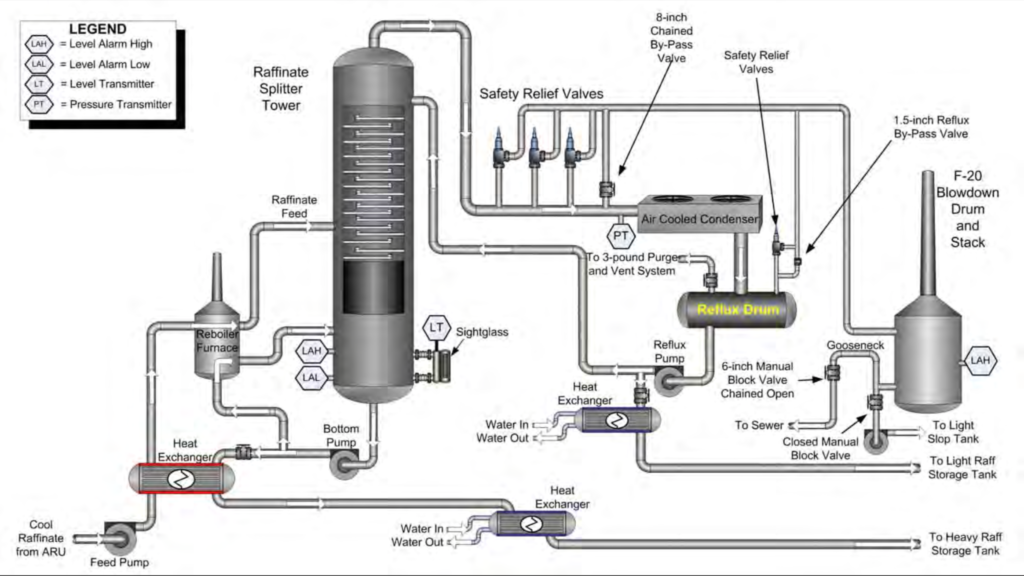
\includegraphics[width=\textwidth]{BP_Texas_City_ISOM_unit.png}
		\caption{Flow diagram of the ISOM. Hydrocarbons were fed into the raffinate splitter, which split the feed into three parts: heavy and light hydrocarbons, and vapors, which went into the heavy storage tank, light storage tank, and the blowdown drum respectively. (cite BP report)}
		\label{fig:ISOMunit}
	\end{figure}
	
	The raffinate splitter, in normal operation, would have around 2m of liquid from its base. This liquid level was controlled by many overlapping safety systems, all of which had one or more major issues that were not acknowledged nor resolved. On the day of the accident, the heavy storage tank was nearly full from the previous night's operation and the level control valve was shut off, cutting the downward flow to the heavy tank. When the raffine splitter was filled the next morning, the liquid level went up many times the safe amount as there was nowhere else for the materials to go. The raffinate splitter tower overflowed when the liquids expand due to the heat during operation, sending liquid hydrocarbons to the blowdown drum, as seen in Figure \ref{fig:incidentdiagram}. As the blowdown drum inevitably overflowed, hot liquid hydrocarbons shot off from the top and flowed through the drain pipes for sewer disposal.
	
	\begin{figure}[H]

		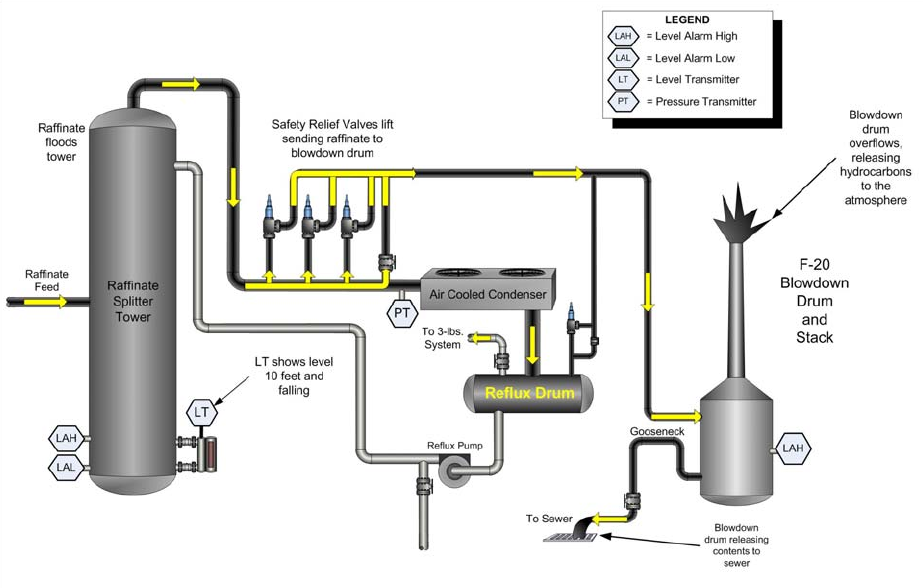
\includegraphics[width=\textwidth]{BP_Texas_City_incident_diagram.png}
		\caption{Incident diagram of the explosion. Compared to the normal flow diagram, the flow to the heavy storage tank was blocked, and raffinate feed overflowed through the top to the blowdown drum. (cite BP report)}
		\label{fig:incidentdiagram}
	\end{figure}
	In the immediate vicinity were workers working on other parts of the ISOM, with their trailers parking right beside the plant, less than 110m away. The closest trailer was only 45m away from the blowdown drum. When the hot liquid hydrocarbons came out of the blowdown drum, the resulting vapor cloud consisting of highly flammable hydrocarbon fumes caused an idle truck engine to overheat and sparked a fire, igniting the vapor cloud. 
	
	The result was a massive explosion that completely destroyed most of the trailers, killing 15 instantly and injuring 180 more, mostly in the trailer areas. The explosion shattered windows three quarters of a mile away and damaged tanks holding hazardous materials such as benzene, leaking them to the environment. The subsequent fire burned up to 19000 $m^2$ of the refinery, causing damages in the millions of dollars. The ISOM itself did not return to normal operation until two years later after sustaining severe damages in the fire. (cite CBS)
	
	The disaster's impact is still felt years after the accident. A study conducted during and after the incident showed that it had led to a decline in the perceived mental and physical health of the people living in the area (cite BMJ). Lawsuits from the victims' families have followed BP, and they have had to pay out 1.6 billion USD in compensation. One notable lawsuit was Eva Rowe's, who demanded justice be brought on the company and forced them to release internal documents showing that they had prior knowledge of the issues plaguing the ISOM. These internal reports later proved to be vital in bringing to light the repeated failures that eventually led to the fatal incident.

	\section*{Engineering failure}
	In 2002, three years before the disaster, Texas City refinery's director ordered an internal report on the mechanical integrity and safety of the plant in response to its obvious decline in the years after the plant's acquisition in 1999. The study concluded that mechanical integrity was an enormous issue, and there were many vulnerabilities in the plant's infrastructure. It then proposed a budget increase of 235 million dollars to rectify these issues, one goal that was eventually not met (cite 2002 study). Many audits and studies followed, but no significant action was taken to conduct maintenance work on the plant, mainly due to continued budget cuts in 2003 and 2005. BP justified these budget cuts as "it had not made a contribution of profit proportionate to its capital consumption," while ignoring that the plant could not operate to its maximum capacity because of its aging and failing infrastructure.
	
	Made two months before the incident but only unveiled a year after the Texas City refinery explosion, another internal report commissioned by BP following other accidents happening in 2004 further detailed the multitudes of existing issues with the plant. This report, called the Telos Report after its author The Telos Group, assessed the "safety behavior and culture" at the plant, specifically the plant's leadership, culture, and safety management. The report displayed how production and budget compliance was valued above all else, and engineers were put under immense pressure to produce while being understaffed and lacking adequate training. It also found various safety issues present on site: alarms were broken, concrete was falling off, and fumes were enveloping the plant. As its final verdict, the Telos Report concluded: “We have never seen a site where the notion ‘I could die today’ was so real” (cite Telos Report).
	
	 The compounding issues hounding the plant carried out a major role in the accident. The raffinate splitter had just been completed, and the start-up process of the plant went into action the night of March 22. One crucial part of this process was the BP Pre-Startup Safety Review procedure consisting of thorough technical and personnel checks, which was not carried out possibly due to a lack of training. The start-up process began with the Night Operator filling the raffinate splitter. Operation through the night meant led to the heavy storage tank being filled completely the morning of March 23 and the flow from the raffinate tower was shut off, but this information was not relayed to the operators working later shifts, once again showing negligence on adhering to safety protocols by the operators involved. 
	 
	  Many of the safety equipments in the raffinate tower were also defective, playing a major part in the accident's progress. When the raffinate splitter tower was refilled in the morning, it overfilled many times its capacity, but this was not caught by any of the engineers involved as the defective level indicators did not give any warning, and the sight glass for manual checking was broken. Had the overfilling of the raffinate tower been caught early, the operators could have shut off the raffinate feed going into the tank, preventing this catastrophe. Another system that could have prevented the issue was the level alarm in the blowdown drum that did not go off even though hydrocarbons were bursting out of its top. Had the engineers known that the blowdown drum was filled with liquid hydrocarbons, they would have realized the issue and shut down the raffinate splitter to deal with the problem.
	  
	  The last egregious issue was a managerial one: the location of the trailers in the plants led to an unnecessary loss of life. In 2002, a site wide temporary siting analysis laid out the allowed parking spaces for trailers. However, work on an adjacent building meant that extra trailers were placed next to the ISOM in 2004, despite the team facilitating this change not having the required knowledge to assess the risk to the trailers in an event of an explosion. In the accident, 12 of the 15 fatalities were contractors inside the trailer situated closest to the ISOM, while the other 8 occupants of that trailer were seriously injured. All of the deaths came from blunt force trauma caused by the equipment in the trailers when the explosion sent a massive shockwave outwards.
	
	\section*{Ethical analysis}
	These engineering failures, in retrospective, were all preventable, yet nothing was done. Through ethical analysis, we can inspect the actions of the involved parties with an ethical framework to  pinpoint the moral failures that led to these devastating consequences and prevent these decisions from repeating. Deontology, or duty ethics, is one of these frameworks: this approach to normative ethics states that actions are morally right as long as they follow a specific set of moral rules. These rules, also known as maxims, must follow two core principles - the universality principle and the reciprocity principle. Based on these maxims, we can categorically define each action as right or wrong independent of their consequences.
	
	The first core principle of duty ethics, the universality principle states that a maxim should only be followed if it can be turned into an universal law. In other words, the maxim must be universally good such that everyone would agree to following it while not ending up contradicting itself. Since these laws are unambiguous and straightforward, however, sometimes they come into conflict with each other. In these cases, the maxims are further divided into prima facie norms (what initially seems to be good) and self-evident norms (what is good when we consider the full context of the situation), where the self-evident norms are usually followed. The second principle in duty ethics is the reciprocity principle, which describes the need for one to respect the rationality of other humans. A maxim can only follow this principle if they do not simply treat humans as a tool to be used for an end. These two principles are the underlying pillars of duty ethics, and actions not following maxims that adhere to these two principles can be considered unethical.
	
	Applied to the Texas City refinery case, deontology can shed light on the morality behind actions taken before, during, and after the incident. The first immediately obvious ethical failure was the inaction of BP and its directors in spite of the internal audits and reports asking for change. Instead of carrying out the required safety upgrade and maintenance work, the company overvalued the importance of production and cited the plant's lack of profits as one of the reason to cut its budget, further undermining its capability to move on from aging equipment (cite 2002 study). Here, BP followed the maxim: "It is unnecessary to follow safety advice from internal reports if it doesn't bring immediate profits." This maxim fails the universality principle, as it is clear that following safety codes is almost always detrimental to a plant's profits as they add more training for their engineers and more redundancy to their core systems. Therefore, internal reports suggesting these safety upgrades would always be ignored, and they would become pointless because no change would ever happen. If this maxim becomes an universal law, no internal investigations would ever be made again, creating a contradiction. 
	\section*{Recommendations}
	\section*{Conclusion}
	\section*{Sources}
	https://www.pbs.org/wgbh/pages/frontline/the-spill/bp-troubled-past/
	https://www.csb.gov/bp-america-refinery-explosion/
	https://people.uvawise.edu/pww8y/Supplement/-ConceptsSup/Work/WkAccidents/BPTxCityFinalReport.pdf
	https://www.nytimes.com/2010/07/13/business/energy-environment/13bprisk.html?pagewanted=all
	https://www.propublica.org/article/blast-at-bp-texas-refinery-in-05-foreshadowed-gulf-disaster
	https://bloximages.newyork1.vip.townnews.com/galvnews.com/content/tncms/assets/v3/editorial/6/cb/6cb6d830-d239-11e4-9afa-2f2f90912f92/5511818abc022.pdf.pdf
	https://www.nytimes.com/2009/10/31/business/31labor.html
	https://jech.bmj.com/content/62/2/106
\end{document}